\documentclass[border=10pt]{standalone}
\usepackage{tikz}
\usetikzlibrary{arrows.meta, positioning}

\definecolor{pastelpurple}{HTML}{6E66BA}
\begin{document}
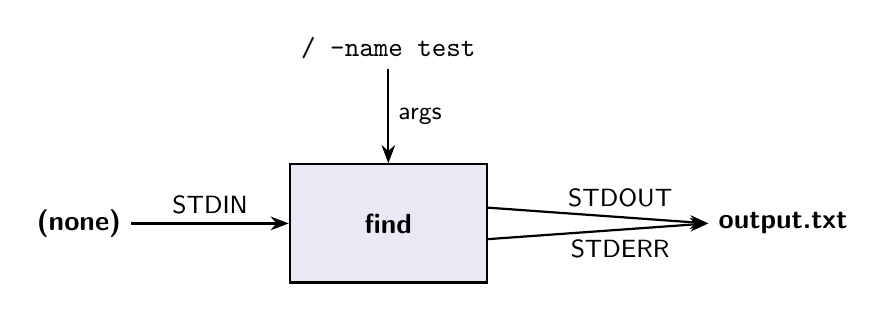
\begin{tikzpicture}[
    >=Stealth,
    thick,
    lbl/.style={font=\sffamily\bfseries},
    arg/.style={font=\ttfamily},
    every edge/.style={draw, ->, thick}
]

% program box
\node[draw, rectangle, minimum width=2.5cm, minimum height=1.5cm, fill=pastelpurple!15, font=\sffamily\bfseries] (program) {find};

% args value above
\node[arg, above=1.2cm of program] (args) {/ -name test};

% unused label on the left
\node[lbl, left=2cm of program] (stdin) {(none)};

% single file on the right
\node[lbl, right=2.8cm of program] (file) {output.txt};

% arrows
\draw[->] (stdin) -- node[above, font=\sffamily\small] {STDIN} (program);
\draw[->] (args) -- node[right, font=\sffamily\small] {args} (program);
\draw[->] (program.east) ++(0,0.2) -- node[above, font=\sffamily\small, pos=0.6] {STDOUT} (file.west);
\draw[->] (program.east) ++(0,-0.2) -- node[below, font=\sffamily\small, pos=0.6] {STDERR} (file.west);

\end{tikzpicture}
\end{document}
